\clearpage
\section{Heatime Data Plots}

\begin{figure}[h]
\centering
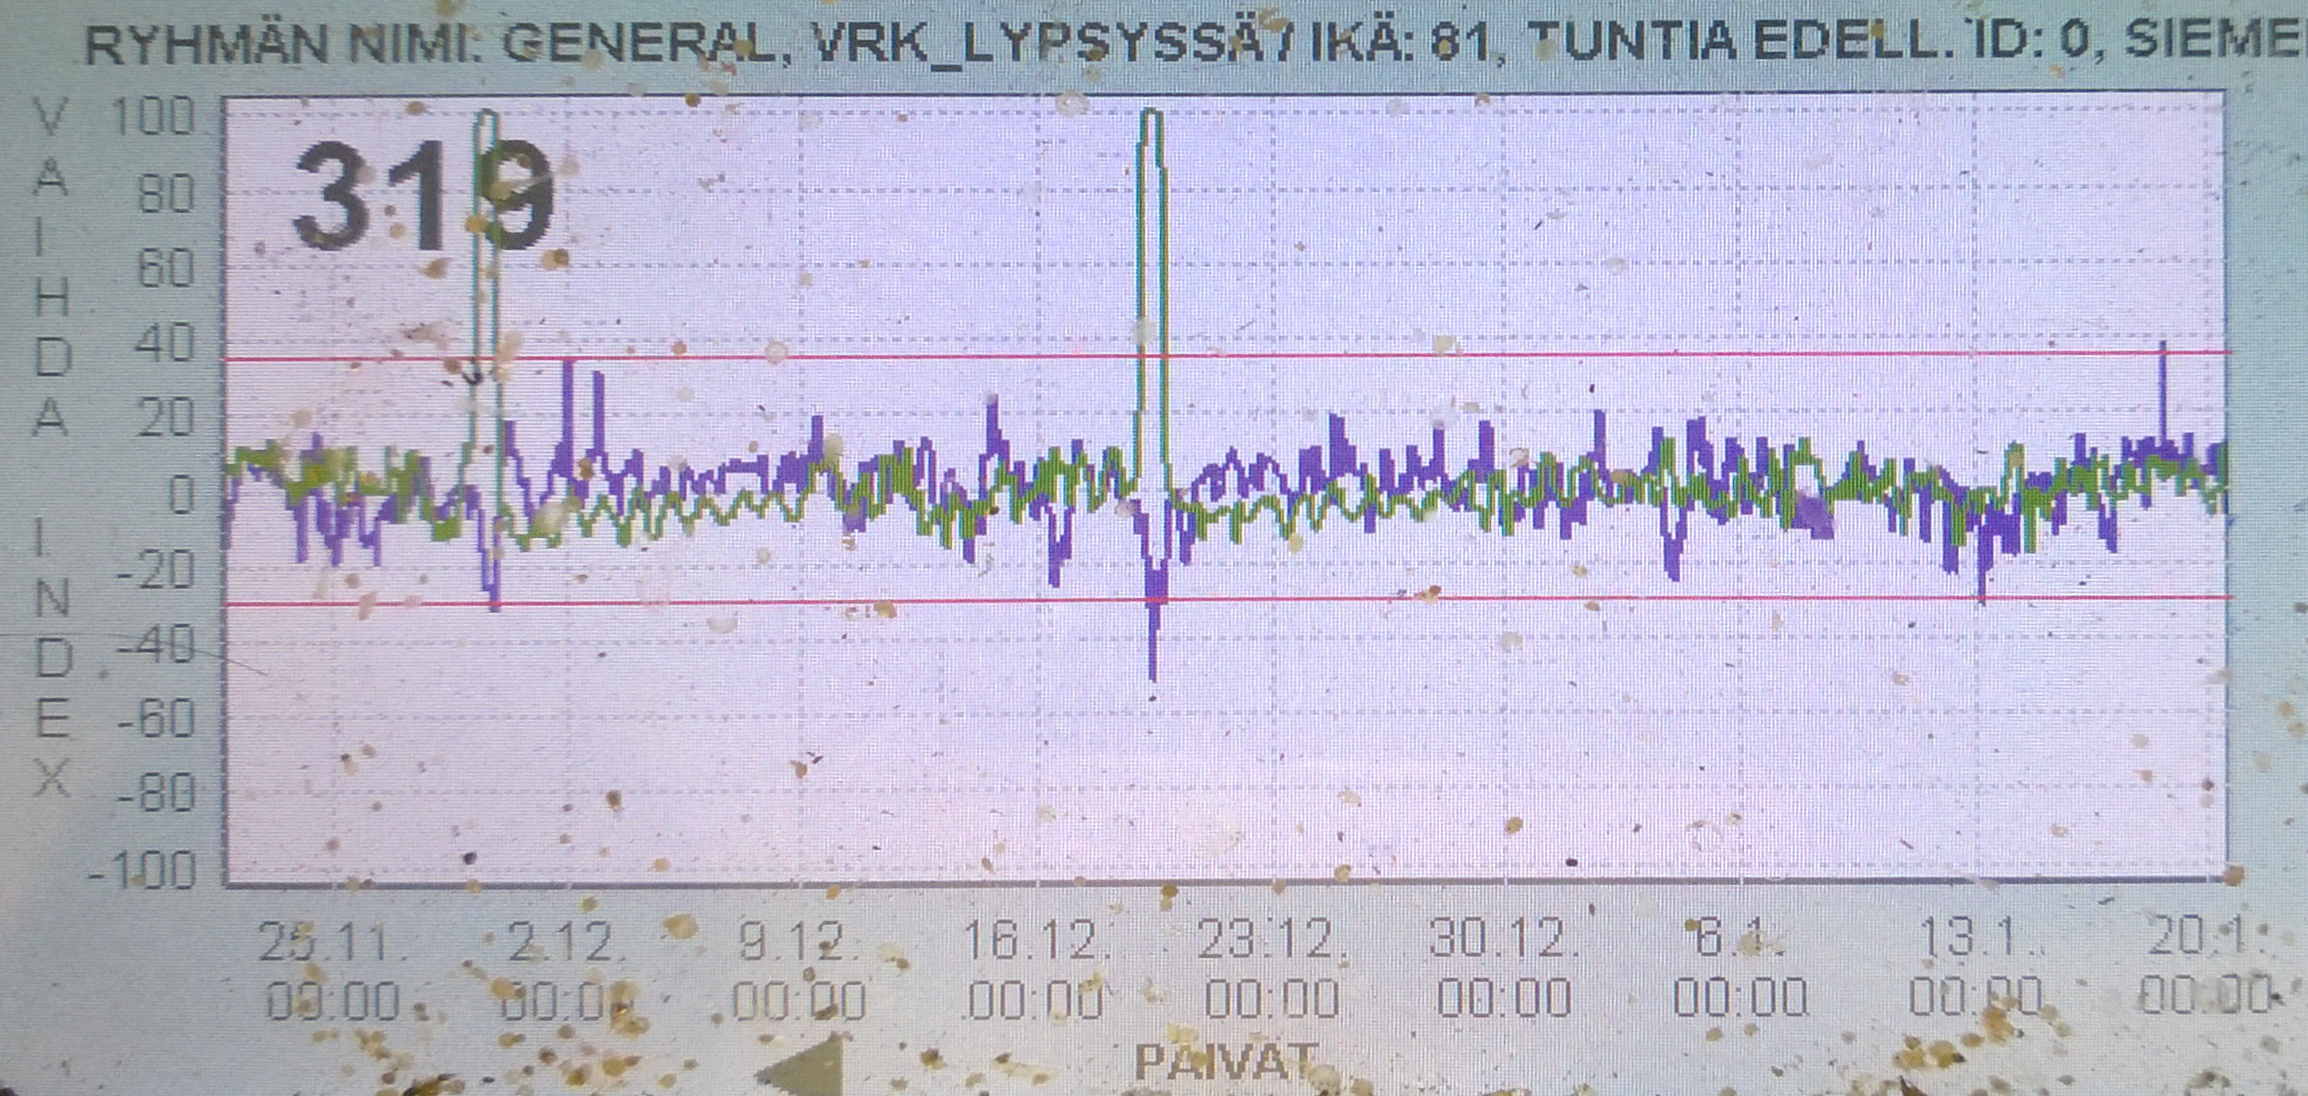
\includegraphics[width = 0.75\textwidth]{figures/heatime_kiima_319}
\caption{The activity data of Heatime system of the cow 319. The cow has had estruses approximately on October the 30\textsuperscript{th} and December the 20\textsuperscript{th}. The latter of the estruses should be detectable in this study, hence it is within our data recording period.}
\label{heatime_kiima_319}
\end{figure}


\begin{figure}[h]
\centering
\includegraphics[width = 0.75\textwidth]{figures/heatime_kiima_9885}
\caption{The activity data of Heatime system of the cow 9885. The cow has had estruses approximately on October the 24\textsuperscript{th}, December the 22\textsuperscript{nd} and January the 4\textsuperscript{th}. Two latter estruses should be detectable in this study, hence they both are within our dat recording period. }
\label{heatime_kiima_9885}
\end{figure}

\begin{figure}[h]
\centering
\includegraphics[width = 0.75\textwidth]{figures/heatime_kiima_767}
\caption{The activity data of Heatime system of the cow 767. The cow has had estruses approximately on January the 21\textsuperscript{st} and February the 13\textsuperscript{th}. The latter of the estruses should be detectable in this study, hence it is within our data recording period.}
\label{heatime_kiima_767_2}
\end{figure}

\begin{figure}[h]
\centering
\includegraphics[width = 0.75\textwidth]{figures/heatime_kiima_787}
\caption{The activity data of Heatime system of the cow 787. The cow has had estruses approximately on January the 19\textsuperscript{th} and February the 10\textsuperscript{th}. The latter of the estruses should detectable in this study, hence it is within our data recording period.}
\label{heatime_kiima_787}
\end{figure}



\clearpage
\section{Raw Accelerometric Data}

\begin{figure}[h]
\centering
\includegraphics[width = 0.75\textwidth]{figures/kiimadata_9885_1.png}
\caption{The raw acceleration data of each axis of the cow 9885. The time frame is scaled around the first detectable estrus period. }
\label{kiimadata_9885_1}
\end{figure}

\begin{figure}[h]
\centering
\includegraphics[width = 0.75\textwidth]{figures/kiimadata_9885_2.png}
\caption{The raw acceleration data of each axis of the cow 9885. The time frame is scaled around the second detectable estrus period. }
\label{kiimadata_9885_2}
\end{figure}

\clearpage
\section{Activity Monitoring Full Results}

\begin{figure}[h]
\centering
\includegraphics[width = 0.75 \textwidth]{figures/ActivityMonitoringCow319.png}
\caption{The plot of the results of the activity measurement algorithm of cow 319. A true positive estrus is detected and no false positive or false negative detection occurred. However, there is a lot of variation when not in estrus. Thus, the risk of false positive and false negative results is plausible.}
\label{ActivityMonitoringCow319}
\end{figure}

\begin{figure}[h]
\centering
\includegraphics[width = 0.75 \textwidth]{figures/ActivityMonitoringCow9885.png}
\caption{The results of activity measurement of the cow 9885. Both of the estruses are detected. However, the difference between the estruses and the rest of the period is insignificant as it was with cow 319. Thus, the possibility of false positive and false negative results exists.}
\label{ActivityMonitoringCow9885}
\end{figure}

\begin{figure}[h]
\centering
\includegraphics[width = 0.75 \textwidth]{figures/ActivityMonitoringCow767.png}
\caption{The plot of the activity measurement results of the cow 767. A true positive estrus is detected and no occurrence of false positives of false negatives. Additionally, the difference between proestrus and rest of the period is obvious. The risk of false positive or false negative results is minor. }
\label{ActivityMonitoringCow767}
\end{figure}

\begin{figure}[h]
\centering
\includegraphics[width = 0.75 \textwidth]{figures/ActivityMonitoringCow787.png}
\caption{The results of activity measurement of the cow 787. The difference between the estrus and rest of the period is most distinct within this algorithm. Thus, the risk of false positive and false negative results is least significant.}
\label{ActivityMonitoringCow787}
\end{figure}

\begin{figure}[h]
\centering
\includegraphics[width = 0.75\textwidth]{figures/redcowactivity2.png}
\caption{The activity plots of the second proestrus of the cow 9885. The figure illustrates the affect of varying the size of the integration window. Wider window increases the amplitude of the estrus and eases the detectability. However, simultaneously it delays the moment of detection. }
\label{integrationwindows}
\end{figure}

\clearpage
\section{Variance Detection Full Results}

\begin{figure}[h]
\centering
\includegraphics[width = 0.75 \textwidth]{figures/VarianceDetectionCow319.png}
\caption{The results of the variance detection algorithm of the cow 319. The estrus on December the 20\textsuperscript{th} is barely detectable. Additionally, algorithm yielded several false positive estruses. Furthermore, the amplitude of the false positives exceeds the true positive.}
\label{VarianceDetectionCow319}
\end{figure}

\begin{figure}[h]
\centering
\includegraphics[width = 0.75 \textwidth]{figures/VarianceDetectionCow9885.png}
\caption{The results of variance detection algorithm of the cow 9885. The true positive estrus is detected on December the 22\textsuperscript{st}. Furthermore, the amplitude difference between the detected estrus and other period is significant. However, the algorithm yield a false negative on January the 4\textsuperscript{th}.}
\label{VarianceDetectionCow9885}
\end{figure}

\begin{figure}[h]
\centering
\includegraphics[width = 0.75 \textwidth]{figures/VarianceDetectionCow767.png}
\caption{The variance detection results of the cow 767. There are multiple false positive detections in the data period. In general, there is no obvious difference between the estrus and non-estrus periods. Nevertheless, a true positive estrus is detected on February the 13\textsuperscript{th}.}
\label{VarianceDetectionCow767}
\end{figure}

\begin{figure}[h]
\centering
\includegraphics[width = 0.75 \textwidth]{figures/VarianceDetectionCow787.png}
\caption{The results of variance detection algorithm of the cow 787. The true positive estrus is detected on February the 10\textsuperscript{th}. However, a false positive detection occurred on February the 21\textsuperscript{st}. Otherwise, the amplitude  difference between estrus and non-estrus periods is obvious.}
\label{VarianceDetectionCow787}
\end{figure}

\begin{figure}[h]
\centering
\includegraphics[width = 0.75 \textwidth]{figures/VarianceDetectionCow319_16frames72seconds.png}
\caption{Reducing the sample size to 16 frames per sample and keeping the sampling interval in 72 seconds yields false positive results with the cow 319}
\label{}
\end{figure}

\begin{figure}[h]
\centering
\includegraphics[width = 0.75 \textwidth]{figures/VarianceDetectionCow767_16frames72seconds.png}
\caption{Reducing the sample size to 16 frames per sample and keeping the sampling interval in 72 seconds yields false positive results with the cow 767}
\label{}
\end{figure}

%------------%

\begin{figure}[h]
\centering
\includegraphics[width = 0.75 \textwidth]{figures/VarianceDetectionCow319_16frames24seconds.png}
\caption{Reducing the sample size to 16 frames and increasing the sampling interval to 24 seconds improves the performance of the variance detection algorithm. Consequently, no false positive results occurs.}
\label{}
\end{figure}

\begin{figure}[h]
\centering
\includegraphics[width = 0.75 \textwidth]{figures/VarianceDetectionCow767_16frames24seconds.png}
\caption{Reducing the sample size to 16 frames and increasing the sampling interval to 24 seconds improves the performance of the variance detection algorithm. Consequently, no false positive results occurs.}
\label{}
\end{figure}


Varying the sampling interval affect the results:


\begin{figure}[h]
\centering
\includegraphics[width = 0.75 \textwidth]{figures/VarianceDetectionCow767_32frames144seconds.png}
\caption{More seldom sampling yield false positive results as seen in this picture.}
\label{}
\end{figure}


\begin{figure}[h]
\centering
\includegraphics[width = 0.75 \textwidth]{figures/VarianceDetectionCow9885_32frames2seconds.png}
\caption{Decreasing the sampling interval does not directly improve the results as it is with the cow 9885. This sampling frequency corresponds approximately continuous sampling. Nevertheless, the results are worse than formerly.}
\label{}
\end{figure}



\begin{figure}[h]
\centering
\includegraphics[width = 0.75 \textwidth]{figures/VarianceDetectionCow767_64frames144seconds.png}
\caption{}
\label{}
\end{figure}

\begin{figure}[htb]
\centering
\includegraphics[width = 0.75 \textwidth]{figures/VarianceDetectionCow319_64frames144seconds.png}
\caption{}
\label{}
\end{figure}

\begin{figure}[h]
\centering
\includegraphics[width = 0.75 \textwidth]{figures/VarianceDetectionCow767_64frames240seconds.png}
\caption{}
\label{}
\end{figure}


\clearpage
\section{Inactivity Detection Full Results}


\begin{figure}[h]
\centering
\includegraphics[width = 0.75 \textwidth]{figures/InactivityDetectionCow319.png}
\caption{The results of the inactivity detection algorithm of the cow 319. The parameters are 336 second delay and \SI{2}{\gram} motion threshold. A true positive estrus is detected on December the 20\textsuperscript{th}. The amplitude of proestrus and non-estrus is significant. }
\label{InactivityDetectionCow319}
\end{figure}


\begin{figure}[h]
\centering
\includegraphics[width = 0.75 \textwidth]{figures/InactivityDetectionCow9885.png}
\caption{The results of inactivity detection algorithm of the cow 9885. The parameters are 336 second delay and \SI{2}{\gram} motion threshold. Both of the estruses are detected as true positive on December the 22\textsuperscript{nd} and January the 4\textsuperscript{th}. No false positive or false negative detection occurred. The amplitude difference between proestrus and non-estrus is obvious.}
\label{InactivityDetectionCow9885}
\end{figure}


\begin{figure}[h]
\centering
\includegraphics[width = 0.75 \textwidth]{figures/InactivityDetectionCow767.png}
\caption{The results of the inactivity detection algorithm of the cow 767. The parameters are 336 second delay and \SI{2}{\gram} motion threshold. A true positive estrus is detected on February the 13\textsuperscript{th}. Additionally, the amplitude of the proestrus differs from none-estrus significantly.}
\label{InactivityDetectionCow767}
\end{figure}

\begin{figure}[h]
\centering
\includegraphics[width = 0.75 \textwidth]{figures/InactivityDetectionCow787.png}
\caption{The results of inactivity detection algorithm of the cow 787. The parameters are 336 second delay and \SI{2}{\gram} motion threshold. A ture positive estrus is detected on February the 11\textsuperscript{th} and no false positives of false negatives occurred. Furthermore, the difference between estrus and other periods is most significant.}
\label{InactivityDetectionCow787}
\end{figure}



\begin{figure}[h]
\centering
\includegraphics[width = 0.75 \textwidth]{figures/InactivityDetectionCow9885_336period05threshold.png}
\caption{}
\label{}
\end{figure}

\begin{figure}[h]
\centering
\includegraphics[width = 0.75 \textwidth]{figures/InactivityDetectionCow9885_336period2_5threshold.png}
\caption{}
\label{}
\end{figure}

\begin{figure}[h]
\centering
\includegraphics[width = 0.75 \textwidth]{figures/InactivityDetectionCow9885_36period.png}
\caption{}
\label{}
\end{figure}

\begin{figure}[h]
\centering
\includegraphics[width = 0.75 \textwidth]{figures/InactivityDetectionCow787_336period05threshold.png}
\caption{}
\label{}
\end{figure}

\begin{figure}[h]
\centering
\includegraphics[width = 0.75 \textwidth]{figures/InactivityDetectionCow787_336period4threshold.png}
\caption{}
\label{}
\end{figure}

\begin{figure}[h]
\centering
\includegraphics[width = 0.75 \textwidth]{figures/InactivityDetectionCow787_336period2_5threshold.png}
\caption{}
\label{}
\end{figure}

\begin{figure}[h]
\centering
\includegraphics[width = 0.75 \textwidth]{figures/InactivityDetectionCow787_36period.png}
\caption{}
\label{}
\end{figure}

\begin{figure}[h]
\centering
\includegraphics[width = 0.75 \textwidth]{figures/InactivityDetectionCow767_336period05threshold.png}
\caption{}
\label{}
\end{figure}

\begin{figure}[h]
\centering
\includegraphics[width = 0.75 \textwidth]{figures/InactivityDetectionCow767_336period4threshold.png}
\caption{}
\label{}
\end{figure}


\begin{figure}[h]
\centering
\includegraphics[width = 0.75 \textwidth]{figures/InactivityDetectionCow767_336period2_5threshold.png}
\caption{}
\label{}
\end{figure}

\begin{figure}[h]
\centering
\includegraphics[width = 0.75 \textwidth]{figures/InactivityDetectionCow767_36period.png}
\caption{}
\label{}
\end{figure}

\begin{figure}[h]
\centering
\includegraphics[width = 0.75 \textwidth]{figures/InactivityDetectionCow319_336period05threshold.png}
\caption{}
\label{}
\end{figure}

\begin{figure}[h]
\centering
\includegraphics[width = 0.75 \textwidth]{figures/InactivityDetectionCow319_336period2_5threshold.png}
\caption{}
\label{}
\end{figure}

\begin{figure}[h]
\centering
\includegraphics[width = 0.75 \textwidth]{figures/InactivityDetectionCow319_36period.png}
\caption{}
\label{}
\end{figure}




%
%\section{Esimerkki liitteestä\label{LiiteA}}
%
%Liitteet eivät ole opinnäytteen kannalta välttämättömiä ja 
%opinnäytteen tekijän on 
%kirjoittamaan ryhtyessään hyvä ajatella pärjäävänsä ilman liitteitä.
%Kokemattomat kirjoittajat, jotka ovat huolissaan
%tekstiosan pituudesta, paisuttavat turhan 
%helposti liitteitä pitääkseen tekstiosan pituuden annetuissa rajoissa.
%Tällä tavalla ei synny hyvää opinnäytettä.   
%
%Liite on itsenäinen kokonaisuus, vaikka se täydentääkin tekstiosaa.
%Liite ei siten ole pelkkä listaus, kuva tai taulukko, vaan 
%liitteessä selitetään aina sisällön laatu ja tarkoitus. 
%
%Liitteeseen voi laittaa esimerkiksi listauksia. Alla on 
%listausesimerkki tämän liitteen luomisesta. 
%
%%% Verbatim-ympäristö ei muotoile tai tavuta tekstiä. Fontti on monospace.
%%% Verbatim-ympäristön sisällä annettuja komentoja ei LaTeX käsittele. 
%%% Vasta \end{verbatim}-komennon jälkeen jatketaan käsittelyä.
%\begin{verbatim}
%	\clearpage
%	\appendix
%	\addcontentsline{toc}{section}{Liite A}
%	\section*{Liite A}
%	...
%	\thispagestyle{empty}
%	...
%	tekstiä
%	...
%	\clearpage
%\end{verbatim}
%
%Kaavojen numerointi muodostaa liitteissä oman kokonaisuutensa:
%\begin{eqnarray}
%d \wedge A  &=& F, \label{liitekaava1}\\
%d \wedge F  &=& 0. \label{liitekaava2}
%\end{eqnarray}
%
%
%\clearpage
%\section{Toinen esimerkki liitteestä\label{LiiteB}}
%
%%% Liitteiden kaavat, taulukot ja kuvat numeroidaan omana kokonaisuutenaan
%
%Liitteissä voi myös olla kuvia, jotka
%eivät sovi leipätekstin joukkoon:
%%% Ympäristön figure parametrit htb pakottavat
%%% kuvan tähän, eikä LaTeX yritä siirrellä niitä
%%% hyväksi katsomaansa paikkaan. 
%%% Ympäristöä center voi käyttää \centering-
%%% komennon sijaan
%%%
%\begin{figure}[htb]
%\begin{center}
%\includegraphics[height=8cm]{kuva2}
%\end{center}
%\caption{Kuvateksti, jossa on liitteen numerointi}
%\label{liitekuva}
%\end{figure}
%%%
%Liitteiden taulukoiden numerointi on kuvien ja kaavojen kaltainen:
%\begin{table}[htb]
%\caption{Taulukon kuvateksti.}
%\label{liitetaulukko}
%\begin{center}
%\fbox{
%\begin{tabular}{lp{0.5\linewidth}}
%9.00--9.55  & Käytettävyystestauksen tiedotustilaisuus (osanottajat
%ovat saaneet sähköpostitse valmistautumistehtävät, joten tiedotustilaisuus
%voidaan pitää lyhyenä).\\
%9.55--10.00 & Testausalueelle siirtyminen
%\end{tabular}}
%\end{center}
%\end{table}
%Kaavojen numerointi muodostaa liitteissä oman kokonaisuutensa:
%\begin{eqnarray}
%T_{ik} &=& -p g_{ik} + w u_i u_k + \tau_{ik},  \label{liitekaava3} \\
%n_i    &=& n u_i + v_i.                      \label{liitekaava4}
%\end{eqnarray}